% su2-rep-theory.tex — Chapter on the SU(2) representation theory
% inputs used throughout the manuscript.
%
% Linked code / Lean:
%   - computations/su2_representations.py
%   - lean/YMGap/RepTheory/   (Casimir constants, character data)

\chapter{\texorpdfstring{$\SUtwo$}{SU(2)} Representation Theory}
\label{ch:su2-rep-theory}

\noindent\emph{Irreducible representations, dimensions, quadratic
Casimirs, characters, and the spectral gap $\Casimir(\tfrac12) =
\tfrac34$ that drives the small-field activity bound.}

This chapter fixes the $\SUtwo$ representation-theoretic data used
throughout the manuscript: the half-integer indexing of irreps, the
dimension and quadratic Casimir formulas, the character on the
maximal torus, and the orthogonality relations.  The single
load-bearing number is the smallest nonzero quadratic Casimir
$\Casimir(\tfrac12) = \tfrac34$, which reappears in
\Cref{ch:small-field-kp} as the spectral-gap coefficient $\clambda$
of the small-field activity bound and propagates through the
$\sigh$-budget to the constructive mass-gap lower bound of
\Cref{ch:mass-gap-theorem}.  The chapter is short, classical, and
self-contained.

\section{Standing convention}
\label{sec:su2-rep-convention}

\marginkey{Physics-spin normalization}%
The Casimir spectrum of $\SUtwo$ depends on the normalization of the
Killing form.  Throughout we adopt the \emph{physics-spin convention}.

\begin{convention}[Generators and Casimir normalization]
\label{conv:physics-spin}
The generators of $\SUtwo$ are
$T_a := \sigma_a / 2$ for $a = 1,2,3$, with $\sigma_a$ the Pauli
matrices.  These satisfy the commutation relations
$[T_a, T_b] = i\,\epsilon_{abc}\, T_c$ and the fundamental-trace
normalization $\mathrm{tr}(T_a T_b) = \tfrac12\,\delta_{ab}$.  The
Laplace--Beltrami operator on $\SUtwo$ with respect to the
bi-invariant metric induced by $-\mathrm{tr}(\cdot\,\cdot)$ on
$\mathfrak{su}(2)$ acts on the spin-$j$ irreducible representation
$V_j$ by multiplication by the quadratic Casimir
\begin{equation}
  \label{eq:casimir-formula}
  \Casimir(j) \;=\; j(j+1) .
\end{equation}
\end{convention}

\begin{infobox}[margin][title=Why this convention]
The physics-spin convention makes the smallest nonzero Casimir
equal to $\tfrac34$ (rather than $\tfrac32$ or $3$ under
dual-Coxeter or full-Killing normalizations).  The choice is
absorbed downstream by the heat-kernel time
$t = 2N/g^2$ of \Cref{ch:heat-kernel}, so the manuscript's
numerical bounds are normalization-independent at the end of the
day.
\end{infobox}

\section{Irreducible representations and Casimirs}
\label{sec:irreps}

\begin{theorem}[Classification of $\SUtwo$ irreps]
\label{thm:irrep-classification}
The isomorphism classes of finite-dimensional unitary irreducible
representations of $\SUtwo$ are in bijection with the half-integers
$j \in \tfrac12\mathbb{N} = \{0, \tfrac12, 1, \tfrac32, \dots\}$.
Each spin-$j$ irrep $V_j$ has
\begin{equation}
  \label{eq:irrep-data}
  \dim V_j \;=\; 2j + 1, \qquad
  \Casimir(j) \;=\; j(j + 1) .
\end{equation}
\end{theorem}

\begin{proof}
Standard; see~\cite{GlimmJaffe1987} Appendix~A or any introduction to
compact Lie groups.  The argument constructs $V_j$ as the spin-$j$
representation of $\mathfrak{su}(2) \cong \mathfrak{so}(3)$, with
highest weight $j$ and lowest weight $-j$; the dimension counts
weights, and the Casimir is computed on a highest-weight vector.
\end{proof}

The first few entries of the Casimir spectrum:
\begin{equation}
  \label{eq:casimir-spectrum}
  \Casimir(0) \;=\; 0, \quad
  \Casimir(\tfrac12) \;=\; \tfrac{3}{4}, \quad
  \Casimir(1) \;=\; 2, \quad
  \Casimir(\tfrac32) \;=\; \tfrac{15}{4}, \quad
  \Casimir(2) \;=\; 6 .
\end{equation}

\marginkey{The spectral gap $\tfrac34$}%
The smallest \emph{positive} Casimir, $\Casimir(\tfrac12) = \tfrac34$,
is the central numerical input of the manuscript.  It is the
spectral gap of the Laplacian on $\SUtwo \setminus \{1\}$ in the
physics-spin convention, and it sets the leading exponential-decay
rate of the heat kernel away from the identity
(\Cref{ch:heat-kernel}).

\begin{lemma}[Spectral gap]
\label{lem:spectral-gap}
For $j > 0$, $\Casimir(j) \ge \Casimir(\tfrac12) = \tfrac34$, with
equality iff $j = \tfrac12$.
\end{lemma}

\begin{proof}
For $j \ge \tfrac12$, $\Casimir(j) - \Casimir(\tfrac12) = j(j+1) -
\tfrac34 = (j - \tfrac12)(j + \tfrac32) \ge 0$, with equality iff
$j = \tfrac12$.
\end{proof}

\section{Characters and the maximal torus}
\label{sec:characters}

Every conjugacy class in $\SUtwo$ has a unique representative on the
maximal torus.  Parameterize the torus by
\begin{equation}
  \label{eq:torus-element}
  t(\theta) \;:=\; \mathrm{diag}\bigl(e^{i\theta/2},\; e^{-i\theta/2}\bigr),
  \qquad \theta \in [0, 2\pi),
\end{equation}
so that $\mathrm{tr}\, t(\theta) = 2\cos(\theta/2)$ ranges over
$[-2, 2]$.  The Weyl integration formula reads
\begin{equation}
  \label{eq:weyl-integration}
  \int_{\SUtwo} f(g)\, dg
  \;=\; \frac{1}{\pi} \int_0^{2\pi} f(t(\theta))\, \sin^2(\theta/2)\, d\theta ,
\end{equation}
where $dg$ is the normalized Haar measure on $\SUtwo$.

\begin{theorem}[Spin-$j$ character]
\label{thm:character}
The character $\chi_j \colon \SUtwo \to \mathbb{C}$ of the spin-$j$
irreducible representation $V_j$, evaluated on the maximal torus, is
\begin{equation}
  \label{eq:character-formula}
  \chi_j(\theta) \;:=\; \chi_j(t(\theta))
  \;=\; \frac{\sin\bigl((2j+1)\,\theta/2\bigr)}{\sin(\theta/2)} .
\end{equation}
At $\theta = 0$ (the identity element, removable singularity),
$\chi_j(0) = 2j + 1 = \dim V_j$.
\end{theorem}

\begin{proof}
Weyl's character formula for $\SUtwo$.  The character is a Laurent
polynomial in $e^{i\theta/2}$ supported on weights from $-j$ to $j$
in integer steps; the explicit sum
$\chi_j(\theta) = \sum_{m = -j}^{j} e^{im\theta}$ telescopes to the
quotient of sines via the geometric-series identity.
\end{proof}

\begin{proposition}[Orthogonality]
\label{prop:character-orthogonality}
The characters $\{\chi_j\}_{j \in \tfrac12\mathbb{N}}$ form an
orthonormal system in $L^2(\SUtwo, dg)$:
\begin{equation}
  \label{eq:character-orthogonality}
  \int_{\SUtwo} \overline{\chi_{j}(g)}\, \chi_{j'}(g)\, dg
  \;=\; \delta_{j, j'} .
\end{equation}
\end{proposition}

\begin{proof}
Standard Peter--Weyl theorem applied to $\SUtwo$.  Compactness of
$\SUtwo$ + finite-dimensional unitary irreps + the normalization of
Haar measure suffice.  See~\cite{GlimmJaffe1987} Appendix~A.
\end{proof}

\begin{mainfigure}
\centering
\begin{tikzpicture}[
  every node/.style={align=center,font=\small},
  axis/.style={->,thick},
  bar/.style={fill=blue!30,draw=blue!60!black,thick},
  hl/.style={fill=red!30,draw=red!60!black,thick},
  scale=1.0
]
  \draw[axis] (-0.4,0) -- (10.4,0) node[right]{$j$};
  \draw[axis] (0,-0.4) -- (0,5.2) node[above]{$\Casimir(j) = j(j+1)$};
  % horizontal grid
  \foreach \y in {1,2,3,4,5} {
    \draw[gray!30,dashed] (0,\y) -- (10.2,\y);
    \node[left,font=\scriptsize] at (-0.05,\y) {$\y$};
  }
  % bars at j=0, 1/2, 1, 3/2, 2, 5/2, 3 (scaled: x = 2*j+0.5)
  \node[below,font=\scriptsize] at (0.5,0) {$0$};
  \node[below,font=\scriptsize] at (1.5,-0.05) {$\tfrac12$};
  \node[below,font=\scriptsize] at (2.5,0) {$1$};
  \node[below,font=\scriptsize] at (3.5,-0.05) {$\tfrac32$};
  \node[below,font=\scriptsize] at (4.5,0) {$2$};
  \node[below,font=\scriptsize] at (5.5,-0.05) {$\tfrac52$};
  \node[below,font=\scriptsize] at (6.5,0) {$3$};
  % Casimir values: 0, 3/4, 2, 15/4, 6, 35/4, 12 -> clip at 5 for display
  \fill[bar] (0.35,0) rectangle (0.65,0.0001);
  \fill[hl]  (1.35,0) rectangle (1.65,0.75);
  \fill[bar] (2.35,0) rectangle (2.65,2.0);
  \fill[bar] (3.35,0) rectangle (3.65,3.75);
  \fill[bar] (4.35,0) rectangle (4.65,5.0);
  \fill[bar] (5.35,0) rectangle (5.65,5.0);
  \fill[bar] (6.35,0) rectangle (6.65,5.0);
  % annotations for last two (clipped)
  \node[above,font=\scriptsize,red!60!black] at (1.5,0.85) {$\tfrac34$};
  \node[above,font=\scriptsize] at (5.5,5.0) {$\tfrac{35}{4}$};
  \node[above,font=\scriptsize] at (6.5,5.0) {$12$};
  % spectral-gap annotation
  \draw[red!70!black,dashed] (0,0.75) -- (10.2,0.75);
  \node[right,font=\scriptsize,red!70!black] at (8.4,0.75) {spectral gap $\tfrac34$};
\end{tikzpicture}
\caption{The first seven entries of the $\SUtwo$ Casimir spectrum
$\Casimir(j) = j(j+1)$ in the physics-spin convention.  The
spin-$\tfrac12$ value $\Casimir(\tfrac12) = \tfrac34$ (highlighted
in red) is the smallest nonzero Casimir; it is the spectral gap
referenced throughout the rest of the manuscript.  Bars for $j \ge 2$
are clipped at the top of the display range.}
\label{fig:casimir-spectrum}
\end{mainfigure}

\section{Use throughout the manuscript}
\label{sec:su2-rep-downstream}

The data of this chapter feed forward as follows.

\begin{itemize}
  \item \Cref{ch:heat-kernel} writes the heat-kernel measure as a
    character expansion
    \begin{equation*}
      K_t(g) \;=\; \sum_{j \in \tfrac12\mathbb{N}}
        (2j + 1)\, \chi_j(g)\, e^{-t\,\Casimir(j)} ,
    \end{equation*}
    so the Casimirs of \eqref{eq:casimir-formula} control the
    exponential decay of each mode.
  \item \Cref{ch:buffer-shell} uses the spectral
    gap $\Casimir(\tfrac12) = \tfrac34$ to drive the uniform-in-$g$
    tail bound on heat-kernel mass away from the identity.
  \item \Cref{ch:small-field-kp} identifies the small-field
    spectral-gap coefficient $\clambda$ with $\Casimir(\tfrac12) =
    \tfrac34$, replacing what was previously a fiducial value
    $\tfrac12$ chosen for order-of-magnitude plausibility.
  \item The constructive mass-gap lower bound $\massgap \ge
    999/1000$ of \Cref{ch:mass-gap-theorem} depends on this
    identification: the $\tfrac34$ Casimir gap (vs.\ the older
    fiducial $\tfrac12$) widens the small-field convergent window
    by $\sim 22\%$ and tightens $\eta_{\mathrm{total}}$ by a factor
    of three at the canonical pilot operating point.
\end{itemize}

\section{Code provenance}
\label{sec:su2-rep-codeanchor}

\begin{itemize}
  \item Python implementation:
    \codepath{computations/su2\_representations.py}.  The module
    exposes the dataclass \codepath{Irrep} carrying both
    \codepath{sympy}-symbolic and \codepath{float}-numeric witnesses
    of the dimension and Casimir, the character function on the
    maximal torus, and a numerical orthogonality verification.
    Tests in \codepath{tests/test\_su2\_representations.py}.
  \item Casimir-spectrum figure:
    \codepath{visualizations/pilot/su2/casimir-spectrum.svg}
    (Python-generated, mirroring \cref{fig:casimir-spectrum}).
  \item Lean formalization: \codepath{lean/YMGap/RepTheory/} and
    \codepath{lean/YMGap/Sheaf/SU2KP.lean::Q'.C2\_oneHalf} for the
    $\Qp$-rational literal $\Casimir(\tfrac12) = \tfrac34$ used by
    downstream small-field machinery.
\end{itemize}
